\section{Power System}

The power source in AAUSHIP is chosen to be LiPo batteries, which is
a type of battery chemistry where the operator take great care in not damaging
the batteries. If care is not taken they might catch on fire, which
cannot easily be extinguished. This can of course be dangerous.

\subsection{Power Harness}
The power system on the ship consists of some somewhat convoluted
wiring harnessed loosely in the hull structures. An single line
diagram is therefor provided to give an overview of the system.

\begin{figure}[htbp]
	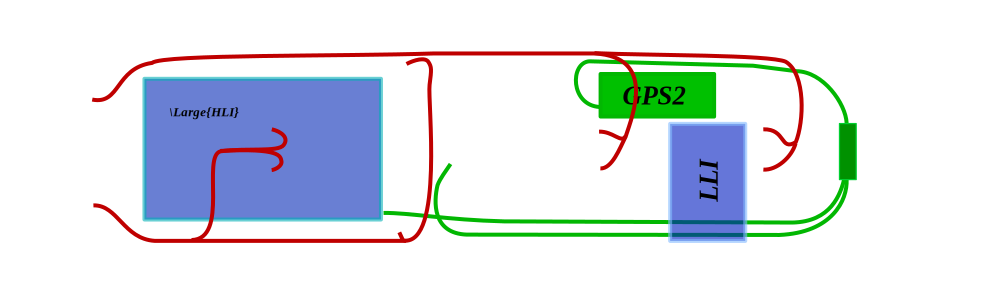
\includegraphics[width=\textwidth]{fig/harness}
	\caption{Power harness system of AAUSHIP}
	\label{fig:harness}
\end{figure}

\begin{figure}[htbp]
	
\includegraphics[width=\textwidth]{fig/mechanical}
	\caption{Overview of the mechanical base components and their
	arrangement. Side view and top view.}
	\label{fig:mechanical}
\end{figure}

\subsection{LiPo Basics}
The LiPo battery packs each consists of four cells in series, which in
the LiPo battery world is called ``4S1P''. One parallel is what you get
when you only have a series connection.

Since each cell is normally not charged individually but across the
output terminals of the battery, every pack with more than one series
cell is equipped with a so called balance port. This is basically a
smaller multiple pin connector that has a connection to each cell,
such that is is possible for a ``balancer'' to discharge cells that is
unbalanced. An unbalanced cell is basically just a cell that does not
have the same voltage as the others.

This balancer is usually run whilst one is charging the main
connections. The purpose is to eliminate the difference that is
inherent in each cell not being exactly the same, such that one cell
does not get overcharged, when charging them in series.

\subsection{LiPo Battery Safety}
\begin{tcolorbox}[colback=yellow!75!,colframe=red]
It is strongly advised not to mess with the LiPo batteries before you
have read and understand how to handle them. A good resource for
learning some basics and safety about LiPo batteries are
\citep{tjintech:lipo-basics} and \citep{tjintech:lipo-safety}.
\end{tcolorbox}
 
